\documentclass[aspectratio=1610]{beamer}
%documentclass[aspectratio=1610, handout]{beamer}
\usepackage[utf8]{inputenc}
\usepackage{ragged2e}
\usepackage{xcolor}
\usepackage[italian]{babel}
\usepackage{multirow}
\usetheme[progressbar=frametitle,titleformat=smallcaps]{metropolis}
\setbeamertemplate{frame numbering}[fraction]
\setbeamercovered{dynamic}
\definecolor{rosso}{RGB}{255, 0, 0}
\definecolor{giallo}{RGB}{254,212,23}
\hypersetup{colorlinks=true,linkcolor=black,urlcolor=rosso}
\setbeamercolor{palette primary}{fg=black, bg=giallo}
\setbeamercolor{background canvas}{bg=white}
\setbeamercolor{normal text}{fg=black}
\setbeamercolor{progress bar}{fg=rosso}
\setbeamercolor{framesubtitle}{fg=rosso}
\setbeamercolor{normal text .dimmed}{fg=giallo}
\setbeamercolor{block title alerted}{fg=rosso, bg=giallo}
\setbeamerfont{caption}{size=\tiny}
\setbeamerfont{caption name}{size=\tiny}
\setlength{\abovecaptionskip}{0pt}
\makeatletter
\metroset{block=fill}
\setlength{\metropolis@progressinheadfoot@linewidth}{1pt} 
\setlength{\metropolis@progressonsectionpage@linewidth}{1pt}
\setlength{\metropolis@titleseparator@linewidth}{1pt}
\makeatother

\title{INTERFACCIA UTENTE E APPLICAZIONI}
\subtitle{5°-6° livello del Sistema Operativo}
\date{}
\institute{\textit{
        Fonti:
        \begin{itemize}
            \item[-] \href{https://www.unimi.it/it/corsi/laurea-triennale/informatica}{Appunti Università degli Studi di Milano}
        \end{itemize}
    }
}

\begin{document}

\begin{frame}[plain, noframenumbering]
    \titlepage
\end{frame}

\section{INTERFACCIA UTENTE}

\begin{frame}{INTERFACCIA UTENTE}
    \begin{columns}
        \column{.5\textwidth}
            \begin{alertblock}{DEFINIZIONE}
                \begin{minipage}{0.97\linewidth}
                    \justifying
                    L'interfaccia utente è il livello del sistema operativo che si occupa di gestire le interazioni tra 
                    l'utente e il sistema operativo, può essere di due tipologie:
                    \begin{itemize}
                        \item \textbf{Command Line Interface (CLI)}: interazione tramite comandi testuali, digitando le istruzioni sulla tastiera.
                        \item \textbf{Graphical User Interface (GUI)}: interazione tramite interfaccia grafica, utilizzando il mouse e le icone per selezionare le opzioni e i comandi.
                    \end{itemize}
                \end{minipage}
            \end{alertblock}
        \column{.5\textwidth}
            \begin{figure}
                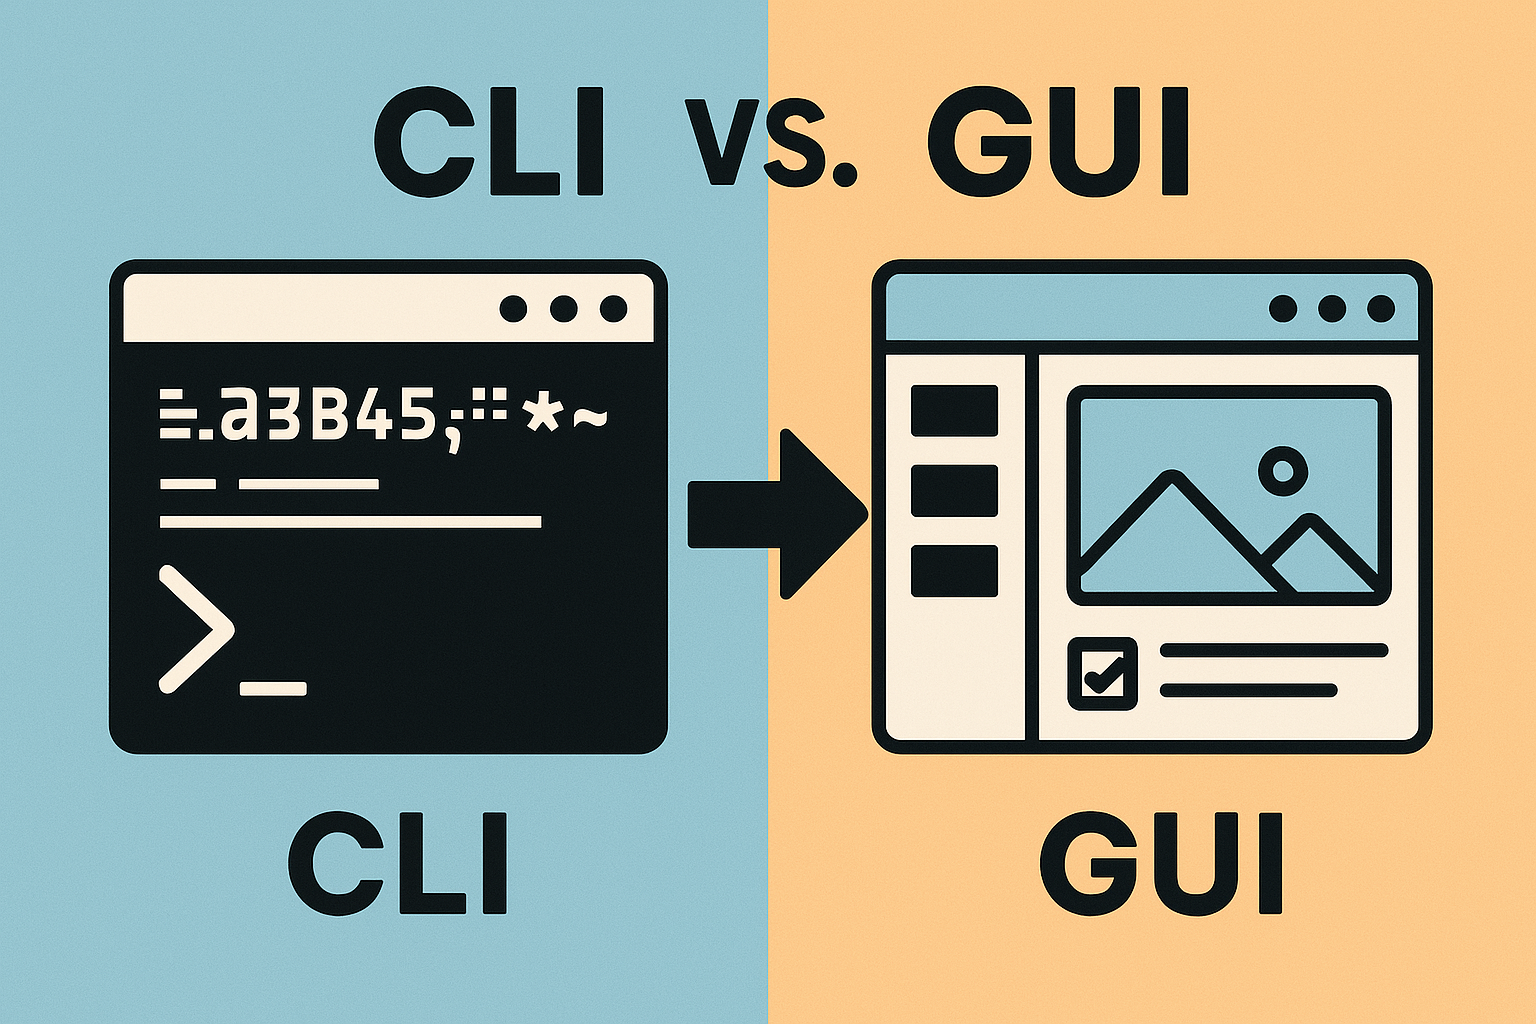
\includegraphics[width=\linewidth]{img/CLIvsGUI.png}
                \caption{{creata con \href{https://chatgpt.com/}{ChatGPT}}}
                \tiny{\textbf{Curiosità}}\\
                \tiny{\href{https://classicreload.com/Windows-1-01.html}{Windows 1.01 del 1985}}\\
                \tiny{\href{https://jamesfriend.com.au/pce-js/}{Classic Macintosh 7.0.1 del 1984}}
            \end{figure}
    \end{columns}
\end{frame}

\end{document}